\documentclass[11pt,openany,oneside]{book}
\usepackage[a4paper,top=25mm,bottom=23mm,left=25mm,right=22mm,headheight=24pt]{geometry}
\usepackage{fontspec}
\setmainfont{DejaVu Serif}
\setsansfont{DejaVu Sans}
\usepackage{amssymb,xcolor,graphicx,array,booktabs,longtable,tabularx,colortbl,enumitem,tikz,tcolorbox,fancyhdr,titlesec,tocloft,hyperref,eso-pic,microtype,listings}
\usetikzlibrary{arrows.meta,positioning,shapes.geometric,calc}
\definecolor{Navy}{HTML}{17365D}
\definecolor{Teal}{HTML}{007F86}
\definecolor{Pale}{HTML}{EAF6F7}
\definecolor{Gold}{HTML}{E3A72F}
\definecolor{Ink}{HTML}{293746}
\definecolor{LightGold}{HTML}{FFF5DD}
\definecolor{SoftGray}{HTML}{F4F6F9}
\definecolor{Coral}{HTML}{D95D50}
\definecolor{Rose}{HTML}{FCE8E6}
\definecolor{Violet}{HTML}{7656A6}
\definecolor{Sky}{HTML}{DCEEFF}
\hypersetup{colorlinks=true,linkcolor=Teal,urlcolor=Teal,pdftitle={Web Developer -- Grade XII},pdfauthor={Vocational Education Textbook}}
\setlist[itemize]{leftmargin=1.5em,itemsep=1.5pt,topsep=2pt,parsep=0pt}
\setlist[enumerate]{leftmargin=1.7em,itemsep=2pt,topsep=2pt,parsep=0pt}
\setlength{\parindent}{0pt}\setlength{\parskip}{3pt}\setlength{\emergencystretch}{3em}
\lstdefinelanguage{PHP}{sensitive=true,morecomment=[l]{//},morecomment=[s]{/*}{*/},morestring=[b]',morestring=[b]",morekeywords={echo,print,if,else,elseif,while,for,foreach,function,return,include,require,isset,empty,global,new,try,catch,throw,public,private,protected,class,true,false,null}}
\lstdefinelanguage{SQL}{morekeywords={SELECT,FROM,WHERE,ORDER,BY,GROUP,INSERT,INTO,VALUES,UPDATE,SET,DELETE,CREATE,DATABASE,TABLE,ALTER,DROP,PRIMARY,KEY,FOREIGN,REFERENCES,NOT,NULL,UNIQUE,DEFAULT,JOIN,LEFT,INNER,ON,AS,COUNT,SUM,AVG,MIN,MAX,GRANT,REVOKE,COMMIT,ROLLBACK},sensitive=false,morecomment=[l]{--},morestring=[b]'}
\lstdefinestyle{webcode}{basicstyle=\ttfamily\small,keywordstyle=\color{Navy}\bfseries,commentstyle=\color{Teal},stringstyle=\color{Violet},numbers=left,numberstyle=\tiny\color{Ink!65},stepnumber=1,numbersep=8pt,showstringspaces=false,breaklines=true,frame=single,rulecolor=\color{Teal!55},backgroundcolor=\color{SoftGray},xleftmargin=2mm,framexleftmargin=2mm,aboveskip=5pt,belowskip=5pt}
\AddToShipoutPictureBG{\begin{tikzpicture}[remember picture,overlay]\draw[Navy!65,line width=.55pt] ([xshift=11mm,yshift=-11mm]current page.north west) rectangle ([xshift=-11mm,yshift=11mm]current page.south east);\draw[Teal,line width=1.6pt] ([xshift=11mm,yshift=-11mm]current page.north west)--([xshift=37mm,yshift=-11mm]current page.north west);\draw[Coral,line width=1.6pt] ([xshift=-11mm,yshift=11mm]current page.south east)--([xshift=-37mm,yshift=11mm]current page.south east);\fill[Gold] ([xshift=11mm,yshift=-11mm]current page.north west) circle (1.1mm);\fill[Violet] ([xshift=-11mm,yshift=11mm]current page.south east) circle (1.1mm);\end{tikzpicture}}
\pagestyle{fancy}\fancyhf{}
\fancyhead[L]{\raisebox{-3.5mm}[0pt][0pt]{\small\bfseries\sffamily\color{Teal} WEB DEVELOPER}}
\fancyhead[R]{\raisebox{-3.5mm}[0pt][0pt]{\small\sffamily\color{Navy} GRADE XII TEXTBOOK}}
\fancyfoot[C]{\tikz[baseline=(n.base)]\node[fill=Teal,draw=Gold,line width=.7pt,text=white,circle,minimum size=7mm,inner sep=1pt,font=\small\bfseries] (n) {\thepage};}
\renewcommand{\headrulewidth}{.5pt}
\renewcommand{\headrule}{\hbox to\headwidth{\color{Gold}\leaders\hrule height \headrulewidth\hfill}}
\fancypagestyle{plain}{\fancyhf{}\fancyhead[L]{\raisebox{-3.5mm}[0pt][0pt]{\small\bfseries\sffamily\color{Teal} WEB DEVELOPER}}\fancyhead[R]{\raisebox{-3.5mm}[0pt][0pt]{\small\sffamily\color{Navy} GRADE XII TEXTBOOK}}\fancyfoot[C]{\tikz[baseline=(n.base)]\node[fill=Teal,draw=Gold,line width=.7pt,text=white,circle,minimum size=7mm,inner sep=1pt,font=\small\bfseries] (n) {\thepage};}\renewcommand{\headrulewidth}{.5pt}\renewcommand{\headrule}{\hbox to\headwidth{\color{Gold}\leaders\hrule height \headrulewidth\hfill}}\renewcommand{\footrulewidth}{0pt}}
\titleformat{\chapter}[display]{\normalfont\sffamily\bfseries\color{Navy}}{\filleft\Large\color{Coral}\chaptername\ \thechapter}{.6ex}{\color{Teal}\LARGE\raggedright}[\vspace{.5ex}\color{Gold}\rule{\textwidth}{.8pt}]
\titlespacing*{\chapter}{0pt}{-8mm}{.5ex}
\titleformat{\section}{\Large\sffamily\bfseries\color{Teal}}{\color{Coral}\thesection}{.7em}{}
\titleformat{\subsection}{\large\sffamily\bfseries\color{Violet}}{\thesubsection}{.7em}{}
\titlespacing*{\section}{0pt}{1.2ex plus .2ex minus .2ex}{.35ex}
\titlespacing*{\subsection}{0pt}{1ex plus .2ex minus .2ex}{.3ex}
\newcommand{\keyterm}[1]{\textbf{\color{Navy}#1}}
\newcommand{\photo}[3]{\begin{center}\begin{tcolorbox}[colback=white,colframe=Teal!70,boxrule=.8pt,arc=1mm,left=2mm,right=2mm,top=2mm,bottom=2mm,width=.88\textwidth]\centering\IfFileExists{images/#1}{\includegraphics[width=.92\linewidth,height=48mm,keepaspectratio]{images/#1}}{\vspace{8mm}\textbf{#2}\par\small Visual example for this topic\vspace{8mm}}\end{tcolorbox}\end{center}{\small\textit{#3}}}
\begin{document}
\begin{titlepage}\thispagestyle{empty}
\begin{tikzpicture}[remember picture,overlay]
\fill[Navy] (current page.north west) rectangle ([yshift=-11.4cm]current page.north east);
\fill[Teal] ([yshift=-11.4cm]current page.north west) rectangle ([yshift=-11.68cm]current page.north east);
\fill[Coral] ([yshift=-11.68cm]current page.north west) rectangle ([yshift=-11.82cm]current page.north east);
\draw[Gold,line width=2pt] ([xshift=22mm,yshift=-20mm]current page.north west)--([xshift=-22mm,yshift=-20mm]current page.north east);
\draw[Gold,line width=1pt] ([xshift=22mm,yshift=-103mm]current page.north west)--([xshift=-22mm,yshift=-103mm]current page.north east);
\end{tikzpicture}
\vspace*{20mm}{\color{white}\rmfamily\bfseries\fontsize{38}{44}\selectfont HANDBOOK\par}
\vspace{5mm}{\color{Gold}\rule{.72\textwidth}{1.2pt}\par}
\vspace{7mm}{\color{white}\sffamily\LARGE Web Developer\par}
\vspace{3mm}{\color{white}\sffamily\large Grade XII -- IT-ITeS Vocational Education\par}
\vfill\begin{center}{\sffamily\Large\bfseries\color{Teal} MySQL \textbullet\ SQL \textbullet\ PHP \textbullet\ Workplace Safety\par}\vspace{4mm}{\sffamily\large\color{Ink} A structured textbook for database development, server-side programming and responsible workplaces.\par}\end{center}
\vfill\begin{center}{\small Developed with reference to the topics in the supplied Grade XII draft study material.\par}\end{center}
\end{titlepage}
\frontmatter
\tableofcontents
\mainmatter

\chapter{Database Management Concepts}
A database becomes useful when information can be stored consistently, found quickly and updated without creating confusion. A school may need student records, a shop may maintain stock and sales, and a web application may keep account details and orders. A database management system (DBMS) provides the tools needed to organise this information and control how people and applications use it.

\photo{computer-room.jpg}{Database infrastructure}{Figure 1.1. A computer room with server equipment illustrates infrastructure that supports database systems. Photograph: StellaAnnie, Wikimedia Commons, CC BY-SA 4.0.}
\section{Data, databases and DBMS}
Data is a recorded value such as a name, date, price or attendance status. A database is an organised collection of related data. A DBMS is software that creates, stores, retrieves and protects that data. MySQL is a widely used relational DBMS; other examples include PostgreSQL, Oracle Database and Microsoft SQL Server.

A database system supports more than storage. It can enforce rules, control access, manage simultaneous users, support backup and recovery, and help applications retrieve only the information they need. These controls reduce the risk of inconsistent or lost records.

\begin{center}
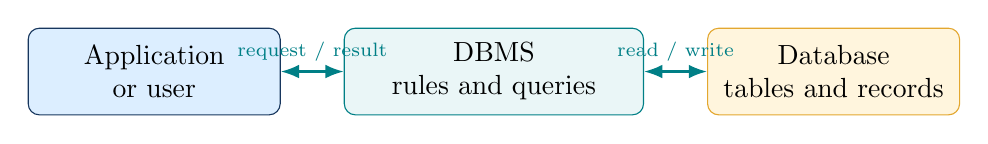
\begin{tikzpicture}[node distance=7mm and 8mm,>=Latex]
\node[draw=Navy,fill=Sky,rounded corners,minimum width=32mm,minimum height=11mm,align=center] (app) {Application\\or user};
\node[draw=Teal,fill=Pale,rounded corners,minimum width=38mm,minimum height=11mm,align=center,right=of app] (dbms) {DBMS\\rules and queries};
\node[draw=Gold,fill=LightGold,rounded corners,minimum width=32mm,minimum height=11mm,align=center,right=of dbms] (data) {Database\\tables and records};
\draw[<->,thick,Teal] (app)--node[above,font=\scriptsize]{request / result}(dbms);
\draw[<->,thick,Teal] (dbms)--node[above,font=\scriptsize]{read / write}(data);
\end{tikzpicture}
\end{center}
\textit{Figure 1.2.} The DBMS mediates between applications and stored data.

\section{Tables, records, fields and keys}
In a relational database, a table stores one kind of entity. Rows represent records; columns represent attributes. A student table might contain student ID, name, class and date of admission. Each column has a data type, and each row should be identifiable in a reliable way.

A \keyterm{primary key} uniquely identifies each row and cannot be missing. A \keyterm{foreign key} links a row to a matching key in another table. A \keyterm{unique constraint} prevents duplicate values in a column or column group. A \keyterm{NOT NULL constraint} requires a value, while a \keyterm{CHECK constraint} can enforce a condition supported by the database engine.

\section{Relational and other database models}
Relational databases organise data in related tables and use SQL to work with it. NoSQL databases use other models, including document, key-value, column-family and graph structures. The appropriate model depends on the shape of the data, consistency needs, access patterns and operational requirements; no single model is best for every application.

\section{File systems and database systems}
A file system stores files and folders. It is appropriate for documents, images and many ordinary files. A DBMS adds structured queries, constraints, relationships and transaction handling that are valuable when many records must be managed together. File storage and databases often work side by side in one application.

\begin{center}
\begin{tabularx}{\textwidth}{p{.24\textwidth}XX}
\toprule
\textbf{Aspect} & \textbf{File-based approach} & \textbf{Database approach}\\\midrule
Structure & Files and folders; format depends on the application & Tables, columns, types and relationships\\
Searching & Often depends on filenames or application-specific logic & SQL queries can filter, sort and join records\\
Integrity & Rules are often implemented separately in code & Constraints can be enforced centrally\\
Concurrent changes & Applications must coordinate carefully & DBMS provides transaction and concurrency controls\\
Security & File permissions and application controls & Database accounts, privileges and application controls\\
Recovery & File backups and application procedures & Backup, logging and database recovery features\\
\bottomrule
\end{tabularx}
\end{center}

\section{Normalisation and data quality}
Normalisation is a way of organising tables to reduce unnecessary repetition and update anomalies. For example, storing a department's address in every employee row means an address change must be repeated in many places. A separate department table allows employees to refer to one department record. Good normalisation begins with clear entities, keys and relationships; it should also reflect actual reporting and performance needs.

\section{Transactions and ACID}
A transaction groups operations that should succeed or fail as a unit. ACID summarises four important properties: Atomicity (all or nothing), Consistency (valid rules remain satisfied), Isolation (concurrent work is controlled), and Durability (committed changes persist according to the system's guarantees). Transactions matter in banking, ordering, stock control and any workflow where partial updates would create a misleading result.

\par\noindent\textbf{Review Questions}\begin{enumerate}[label=\arabic*.,leftmargin=1.8em,itemsep=2pt,topsep=2pt]
\item Define DBMS and give two examples.
\item Distinguish a row from a column.
\item Explain primary and foreign keys.
\item State two advantages and two limitations of a file-based approach.
\item What does each ACID property protect?
\end{enumerate}

\chapter{Structured Query Language and MySQL}
SQL is used to define database structures, retrieve records, change data and manage access. Although database products differ in some details, the basic ideas of tables, filtering, sorting, joins and constraints are widely shared.

\photo{sql-programming.jpg}{SQL and programming code}{Figure 2.1. A code screen illustrates the syntax used to write and review database queries. Photograph: Lorenzo Cafaro, Wikimedia Commons, CC0 1.0.}
\section{Main categories of SQL commands}
\begin{itemize}
\item \textbf{DDL (Data Definition Language):} CREATE, ALTER and DROP define or change database objects.
\item \textbf{DML (Data Manipulation Language):} INSERT, UPDATE and DELETE change records.
\item \textbf{DQL (Data Query Language):} SELECT retrieves information; this label is often used for query statements.
\item \textbf{DCL (Data Control Language):} GRANT and REVOKE manage privileges.
\item \textbf{TCL (Transaction Control Language):} COMMIT and ROLLBACK manage transaction outcomes.
\end{itemize}

\section{Creating a database and table}
The following examples use MySQL-style syntax. Run them in a practice database, not against real records.

\begin{lstlisting}[style=webcode,language=SQL]
CREATE DATABASE training_centre;
USE training_centre;

CREATE TABLE students (
  student_id INT PRIMARY KEY,
  full_name VARCHAR(100) NOT NULL,
  course_name VARCHAR(80),
  marks DECIMAL(5,2) CHECK (marks >= 0 AND marks <= 100)
);
\end{lstlisting}
Choose data types that fit the values. INT is suitable for whole numbers; VARCHAR stores variable-length text; DATE stores a calendar date; DECIMAL is appropriate for exact decimal quantities such as money. Avoid storing every value as text when calculations, sorting or validation matter.

\section{Retrieving and filtering data}
SELECT names the columns to return. WHERE filters rows, ORDER BY sorts the result, and LIMIT can restrict the number of returned rows in MySQL.

\begin{lstlisting}[style=webcode,language=SQL]
SELECT student_id, full_name, marks
FROM students
WHERE marks >= 60
ORDER BY marks DESC
LIMIT 10;
\end{lstlisting}
Use explicit column names rather than relying on SELECT * in long-lived application queries. Explicit selections make the expected output easier to review and reduce accidental exposure when a table gains new columns.

\section{Adding, updating and deleting records}
\begin{lstlisting}[style=webcode,language=SQL]
INSERT INTO students (student_id, full_name, course_name, marks)
VALUES (101, 'Ananya Rao', 'Web Development', 86.50);

UPDATE students
SET marks = 88.00
WHERE student_id = 101;

DELETE FROM students
WHERE student_id = 101;
\end{lstlisting}
UPDATE and DELETE should be used with particular care. Before running a change, check the WHERE condition with a SELECT query and confirm that it identifies exactly the intended records. In real systems, use appropriate permissions, backups and transactions.

\section{Functions, grouping and aggregation}
SQL functions can transform values or summarise a set of records. String functions include UPPER, LOWER, CONCAT and LENGTH; numeric functions include ROUND, CEIL, FLOOR and ABS; date functions depend on the DBMS. Aggregate functions such as COUNT, SUM, AVG, MIN and MAX calculate a summary across rows.

\begin{lstlisting}[style=webcode,language=SQL]
SELECT course_name,
       COUNT(*) AS learner_count,
       ROUND(AVG(marks), 2) AS average_marks
FROM students
GROUP BY course_name
ORDER BY average_marks DESC;
\end{lstlisting}
GROUP BY creates groups for aggregation. HAVING filters groups after aggregation, while WHERE filters rows before grouping. NULL values require care: most aggregate functions ignore NULL inputs, and comparisons with NULL use IS NULL or IS NOT NULL rather than ordinary equality.

\section{Joins and relationships}
A JOIN combines rows from related tables. An INNER JOIN returns matching rows. A LEFT JOIN retains every row from the left table and includes matching data from the right where available. Joins are easier to reason about when key columns are named clearly and their relationships are documented.

\begin{lstlisting}[style=webcode,language=SQL]
SELECT s.full_name, c.course_title
FROM students AS s
INNER JOIN courses AS c
  ON s.course_id = c.course_id;
\end{lstlisting}

\section{Installation and safe database practice}
For learning, use the official MySQL Community Edition download and follow current installation instructions for your operating system. A typical setup may include MySQL Server and a client such as MySQL Workbench. Create a dedicated practice account, use a strong password, keep the server local while learning, and do not expose the database port to the public internet without a carefully designed security plan.

\par\noindent\textbf{Review Questions}\begin{enumerate}[label=\arabic*.,leftmargin=1.8em,itemsep=2pt,topsep=2pt]
\item Compare DDL and DML.
\item What is the purpose of a primary key?
\item Write a query to sort marks from highest to lowest.
\item Explain the difference between WHERE and HAVING.
\item Compare INNER JOIN and LEFT JOIN.
\item Why should UPDATE and DELETE statements be checked before execution?
\end{enumerate}

\chapter{SQL Functions and Data Handling}
Functions help queries express common calculations without requiring every operation to be performed manually outside the database. A function accepts a value or expression and returns a result. Exact names and behaviour can differ across database products, so check the documentation for the system in use.

\section{String functions}
UPPER and LOWER change letter case, CONCAT joins text, LENGTH reports the length according to the DBMS's rules, and TRIM removes surrounding whitespace. SUBSTRING returns part of a string. These operations are useful for formatting output, preparing search values and producing reports. They should not be used as a substitute for storing clean, well-validated data.

\begin{lstlisting}[style=webcode,language=SQL]
SELECT UPPER(full_name) AS display_name,
       LENGTH(full_name) AS name_length
FROM students;
\end{lstlisting}

\section{Numeric functions}
ABS returns a non-negative magnitude, ROUND rounds a number to a specified precision, and CEIL/FLOOR round upward/downward to integer boundaries. Check the effect of rounding before using it in financial or assessment calculations; the displayed value and stored value are not always the same.

\section{Date and time functions}
Date functions can extract parts of a date, compare dates, format a value or calculate intervals. MySQL provides functions such as CURDATE(), NOW(), YEAR() and \texttt{DATE\_FORMAT()}. Other SQL systems may use different names or arguments. Store dates using date/time types when possible, rather than ambiguous strings such as 03/04/25.

\section{Aggregate functions and NULL values}
COUNT counts rows or non-NULL values depending on its argument; SUM totals numeric values; AVG computes a mean; MIN and MAX return the smallest and largest values. NULL means that a value is unknown or absent, not zero and not an empty string. Queries should handle missing values intentionally.

\begin{lstlisting}[style=webcode,language=SQL]
SELECT COUNT(*) AS total_records,
       COUNT(marks) AS records_with_marks,
       AVG(marks) AS mean_marks,
       MIN(marks) AS lowest_marks,
       MAX(marks) AS highest_marks
FROM students;
\end{lstlisting}

\section{Permissions and transactions}
GRANT assigns permitted actions to a database account; REVOKE removes permissions. Follow least privilege: give each account only the access it needs. COMMIT confirms a transaction and ROLLBACK abandons uncommitted changes. Transaction support and behaviour depend on the storage engine and the operations being performed.

\par\noindent\textbf{Review Questions}\begin{enumerate}[label=\arabic*.,leftmargin=1.8em,itemsep=2pt,topsep=2pt]
\item Give examples of string and numeric functions.
\item Compare COUNT(*) with COUNT(column).
\item Why should dates be stored using date types?
\item What is NULL?
\item Explain least privilege in database access.
\end{enumerate}

\chapter{Introduction to PHP and Server-Side Scripting}
PHP is a server-side scripting language often used to create dynamic web pages and web services. The server executes PHP code and sends a response to the browser. Visitors normally receive the resulting HTML, not the server's PHP source. PHP can process form input, apply application rules, communicate with databases and generate a response.

\photo{php-code.jpg}{Server-side source code}{Figure 4.1. Server-side scripts are written and tested in a programming environment. Photograph: Martin Vorel, Wikimedia Commons, CC BY-SA 4.0.}
\section{How a PHP request works}
\begin{center}
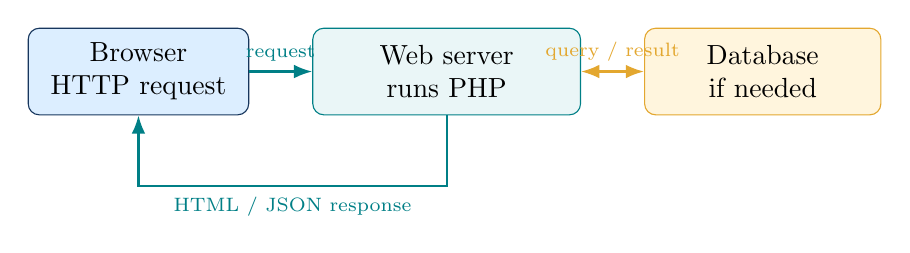
\begin{tikzpicture}[node distance=7mm and 8mm,>=Latex]
\node[draw=Navy,fill=Sky,rounded corners,minimum width=28mm,minimum height=11mm,align=center] (browser) {Browser\\HTTP request};
\node[draw=Teal,fill=Pale,rounded corners,minimum width=34mm,minimum height=11mm,align=center,right=of browser] (php) {Web server\\runs PHP};
\node[draw=Gold,fill=LightGold,rounded corners,minimum width=30mm,minimum height=11mm,align=center,right=of php] (db) {Database\\if needed};
\draw[->,thick,Teal] (browser)--node[above,font=\scriptsize]{request}(php);
\draw[<->,thick,Gold] (php)--node[above,font=\scriptsize]{query / result}(db);
\draw[->,thick,Teal] (php.south) -- ++(0,-9mm) -| node[pos=.25,below,font=\scriptsize]{HTML / JSON response} (browser.south);
\end{tikzpicture}
\end{center}
\textit{Figure 4.2.} A typical request-response path for a server-side application.

\section{Running a first PHP script}
Use a supported PHP installation or a local development bundle, and follow the current official installation instructions. Save the following as \texttt{hello.php} in the configured project directory and open it through the local development server.

\begin{lstlisting}[style=webcode,language=PHP]
<?php
$course = "Web Development";
echo "<h1>Welcome to " . htmlspecialchars($course, ENT_QUOTES, 'UTF-8') . "</h1>";
?>
\end{lstlisting}
PHP variables begin with a dollar sign. Statements commonly end with a semicolon. The \texttt{echo} construct outputs content. When displaying user-controlled text inside HTML, escape it for the correct output context; escaping is a security control, not just a formatting choice.

\section{Variables, types and operators}
Variables hold values such as strings, integers, floating-point numbers, booleans, arrays and objects. PHP is dynamically typed, but developers should still validate input and make assumptions clear. Arithmetic operators calculate values; comparison operators compare values; logical operators combine conditions. Use strict comparisons where appropriate and avoid depending on surprising type conversions.

\section{Conditions and loops}
\begin{lstlisting}[style=webcode,language=PHP]
$marks = 74;
if ($marks >= 80) {
    echo "Excellent";
} elseif ($marks >= 50) {
    echo "Pass";
} else {
    echo "Needs more practice";
}
\end{lstlisting}
Conditions allow code to choose between actions. Loops repeat work while a condition holds or for each item in a collection. Every loop needs a sensible stopping condition so that it does not run forever.

\section{Forms and request data}
HTML forms commonly submit data with GET or POST. GET data is typically included in the URL and is suitable for retrieval requests; POST sends data in the request body and is often used for changes. POST does not automatically make data private or safe: use HTTPS, validation, access control and appropriate request protections.

\begin{lstlisting}[style=webcode,language=PHP]
<?php
if ($_SERVER['REQUEST_METHOD'] === 'POST') {
    $name = trim($_POST['name'] ?? '');
    if ($name === '') {
        echo "Please enter a name.";
    } else {
        echo "Received a valid name.";
    }
}
?>
\end{lstlisting}
The example demonstrates basic checking only. A real form should include a suitable HTML form, a clear label, server-side validation, CSRF protection where relevant, safe output encoding and meaningful error handling.

\par\noindent\textbf{Review Questions}\begin{enumerate}[label=\arabic*.,leftmargin=1.8em,itemsep=2pt,topsep=2pt]
\item What is server-side scripting?
\item Describe the journey of an HTTP request to a PHP server.
\item What is the difference between GET and POST?
\item Why should user-provided text be escaped before it is inserted into HTML?
\end{enumerate}

\chapter{PHP Arrays, Strings and Functions}
\section{Arrays}
An array stores several values under one variable. An indexed array uses numeric keys, an associative array uses named keys, and a multidimensional array contains arrays inside another array. Select the structure that best represents the data.

\begin{lstlisting}[style=webcode,language=PHP]
$courses = ["HTML", "CSS", "JavaScript"];
$learner = [
    "name" => "Ananya",
    "course" => "Web Development",
    "completed" => true
];

foreach ($courses as $course) {
    echo htmlspecialchars($course, ENT_QUOTES, 'UTF-8') . "<br>";
}
\end{lstlisting}
Array functions can sort values, count elements, test for keys and transform data. Be mindful that some sorting functions reindex numeric keys, while others preserve key associations. Check the function's documented behaviour before depending on the original order.

\section{Working with strings}
String operations can trim extra spaces, change letter case, find a substring, split text or join pieces. When processing input, consider empty strings, unexpected encodings and very long values. A value should be checked according to its intended meaning, not merely accepted because it is a string.

\section{Functions and parameters}
A function gives a name to a reusable task. Parameters receive input, and a return value communicates a result. Small functions are easier to test, reuse and maintain than long blocks that mix unrelated responsibilities.

\begin{lstlisting}[style=webcode,language=PHP]
function calculateAverage(array $scores): ?float {
    if (count($scores) === 0) {
        return null;
    }
    return array_sum($scores) / count($scores);
}

$average = calculateAverage([70, 80, 90]);
\end{lstlisting}
PHP passes values by value by default; a parameter can be explicitly passed by reference using an ampersand in its declaration. References should be used only when changing the caller's variable is part of the function's intended behaviour. Recursive functions call themselves and must have a base case to stop the recursion.

\section{Server variables and HTTP headers}
The \texttt{\$\_SERVER} superglobal provides request and server information, such as the request method and script path. Values should not be blindly trusted as proof of identity or permission. HTTP headers communicate metadata and response instructions. Header operations must be sent before body output, and redirects should be followed by an exit where appropriate.

\section{Error handling and maintainability}
Use clear names, consistent formatting, comments that explain intent, and functions with a focused purpose. During development, errors can be logged for diagnosis. Production systems should avoid showing stack traces, secrets or internal paths to visitors. Logs should not unnecessarily contain passwords, session tokens or sensitive personal information.

\par\noindent\textbf{Review Questions}\begin{enumerate}[label=\arabic*.,leftmargin=1.8em,itemsep=2pt,topsep=2pt]
\item Compare indexed and associative arrays.
\item What is the purpose of a foreach loop?
\item Explain function parameters and return values.
\item What is a base case in recursion?
\item Why should internal error details not be displayed to every visitor?
\end{enumerate}

\chapter{PHP and MySQL Database Applications}
A web application often needs to save and retrieve information. PHP can connect to MySQL, send queries and use the returned rows to generate a response. The connection, query and output stages all need careful error handling and security controls.

\photo{server-rack.jpg}{Application and server infrastructure}{Figure 6.1. Web applications depend on server systems to process requests and access stored data. Photograph: Ricardo Moctezuma López / ronK, Wikimedia Commons, CC BY-SA 2.5.}
\section{Connection choices}
Modern PHP applications commonly use PDO or MySQLi. Both support prepared statements. PDO offers a consistent interface across supported database drivers; MySQLi is designed for MySQL-compatible databases. Use the interface supported by the project and keep credentials outside public source files, for example in environment configuration that is not committed to a repository.

\section{Prepared statements}
Never build a query by joining untrusted input directly into SQL text. Prepared statements separate the query structure from the supplied values and help prevent SQL injection.

\begin{lstlisting}[style=webcode,language=PHP]
<?php
$pdo = new PDO(
    'mysql:host=127.0.0.1;dbname=training_centre;charset=utf8mb4',
    getenv('DB_USER'),
    getenv('DB_PASSWORD'),
    [PDO::ATTR_ERRMODE => PDO::ERRMODE_EXCEPTION]
);

$stmt = $pdo->prepare(
    'SELECT student_id, full_name FROM students WHERE student_id = :id'
);
$stmt->execute(['id' => $studentId]);
$student = $stmt->fetch(PDO::FETCH_ASSOC);
?>
\end{lstlisting}
This is a learning pattern, not a complete production configuration. The variable \texttt{\$studentId} must be validated, the credentials must be configured securely, and exceptions should be handled by the application without exposing sensitive details to the browser.

\section{Create, read, update and delete}
CRUD describes four common data operations: create a record, read records, update existing information and delete records. Each operation should verify that the user is authorised to perform it. Deleting records may require confirmation, audit logging or a retention process depending on the system's requirements.

\section{SQL injection}
SQL injection occurs when untrusted input is interpreted as part of a query's executable SQL syntax. It may expose data, bypass checks or modify records. Prepared statements are the primary defence for values; least-privilege database accounts, validation, safe error handling and security testing add further protection. Escaping alone is not a substitute for prepared statements.

\section{Output encoding and sessions}
When displaying text in HTML, use context-appropriate output encoding, such as \texttt{htmlspecialchars} for ordinary HTML text. Authentication systems should use secure session settings, regenerate session identifiers after login, enforce permissions on the server and protect sensitive actions. Hiding a button in the browser is not authorisation.

\section{A responsible development checklist}
\begin{itemize}
\item Use a separate database account with only the privileges needed.
\item Store credentials in environment variables or a protected configuration system.
\item Use prepared statements for values in SQL queries.
\item Validate input on the server and encode output for its context.
\item Use HTTPS for real deployments and protect sessions.
\item Log useful security events without recording secrets.
\item Back up data and test recovery procedures.
\end{itemize}

\par\noindent\textbf{Review Questions}\begin{enumerate}[label=\arabic*.,leftmargin=1.8em,itemsep=2pt,topsep=2pt]
\item Name two PHP interfaces used with MySQL.
\item How do prepared statements reduce SQL injection risk?
\item What do CRUD operations mean?
\item Why is output encoding necessary?
\item Give four checks to complete before a database-backed form is released.
\end{enumerate}

\chapter{Productivity, Quality and Professional Work Habits}
Productivity is not simply completing a large number of tasks. Good work is accurate, useful and delivered with appropriate use of time and resources. In a software workplace, productivity improves when requirements are understood, tasks are prioritised, tools are maintained, communication is clear and defects are found early.

\photo{workstation.jpg}{Organised computer workspace}{Figure 7.1. A workstation should be kept organised so equipment and materials can be used safely. Photograph: Frederick Noronha, Wikimedia Commons, CC BY-SA 4.0.}
\section{Planning and prioritising}
Break large assignments into smaller tasks with clear outcomes. Estimate the effort, identify dependencies and reserve time for review. A simple task board can show work that is planned, in progress, waiting for review and complete. When priorities change, communicate the impact rather than silently missing a deadline.

\section{Quality and continuous improvement}
Quality means meeting agreed requirements reliably. Use checklists, peer review, testing and documented procedures. When an error occurs, look for the cause and improve the process instead of focusing only on blame. Useful measures might include defects found after release, rework, task completion and customer feedback; a single metric rarely tells the whole story.

\section{Communication and teamwork}
Share information in a clear and respectful way. Confirm important instructions, record decisions and raise risks early. When giving feedback, describe the observed issue, its impact and a practical next step. Protect confidential information and use approved channels for work discussions.

\section{Managing digital work responsibly}
Organise files with meaningful names, keep versions under control, back up important work and avoid saving confidential material in unapproved locations. Lock the screen when stepping away, use strong authentication and report suspicious messages or unexpected access requests.

\par\noindent\textbf{Review Questions}\begin{enumerate}[label=\arabic*.,leftmargin=1.8em,itemsep=2pt,topsep=2pt]
\item Distinguish productivity from simply working faster.
\item Give three methods for improving quality.
\item Why should a project risk be reported early?
\item List four habits that support responsible digital work.
\end{enumerate}

\chapter{Health and Safety Procedures in the Workplace}
A safe workplace is created through planning, training, suitable equipment and shared responsibility. Hazards may be physical, electrical, ergonomic, chemical, environmental or psychosocial. Identifying a hazard early gives people a chance to remove it or reduce the risk before someone is harmed.

\photo{ergonomic-workstation.png}{Ergonomic computer workstation}{Figure 8.1. An ergonomic workstation supports comfortable computer use and reduces avoidable strain. Illustration: Marcel Kollmar and Partynia, Wikimedia Commons, CC BY-SA.}
\section{Hazard and risk}
A hazard is something that can cause harm. Risk considers how likely that harm is and how serious it could be. A loose cable across a walkway is a hazard; the risk increases when people regularly walk through the area and could trip. Report hazards promptly and follow the organisation's safety procedure.

\section{Hierarchy of controls}
Where possible, remove the hazard first. If elimination is not practical, consider substituting a safer option, using engineering controls, improving administrative procedures and using personal protective equipment where required. PPE is important but should not be the only control when more effective options are available.

\begin{center}
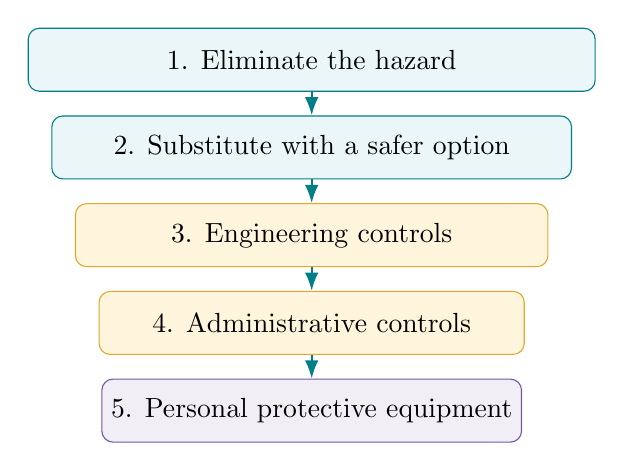
\begin{tikzpicture}[node distance=3mm,>=Latex]
\node[draw=Teal,fill=Pale,rounded corners,minimum width=72mm,minimum height=8mm,align=center] (a) {1. Eliminate the hazard};
\node[draw=Teal,fill=Pale,rounded corners,minimum width=66mm,minimum height=8mm,align=center,below=of a] (b) {2. Substitute with a safer option};
\node[draw=Gold,fill=LightGold,rounded corners,minimum width=60mm,minimum height=8mm,align=center,below=of b] (c) {3. Engineering controls};
\node[draw=Gold,fill=LightGold,rounded corners,minimum width=54mm,minimum height=8mm,align=center,below=of c] (d) {4. Administrative controls};
\node[draw=Violet,fill=Violet!10,rounded corners,minimum width=48mm,minimum height=8mm,align=center,below=of d] (e) {5. Personal protective equipment};
\draw[->,thick,Teal] (a)--(b);\draw[->,thick,Teal] (b)--(c);\draw[->,thick,Teal] (c)--(d);\draw[->,thick,Teal] (d)--(e);
\end{tikzpicture}
\end{center}
\textit{Figure 8.2.} The hierarchy of controls prioritises stronger ways of reducing risk.

\section{Computer-work ergonomics}
Adjust the chair, desk and screen so the body can remain in a comfortable, neutral position. Keep frequently used items within easy reach, avoid glare and take regular short movement breaks. Repeated discomfort, headaches or eye strain should be reported and addressed rather than treated as an unavoidable part of computer work.

\section{Electrical safety and emergency response}
Do not use damaged plugs, exposed wires or overloaded extension boards. Keep liquids away from electrical equipment and never attempt repairs beyond your training or authorisation. Know emergency exits, alarms, first-aid arrangements and reporting contacts. In an emergency, follow local procedures and contact trained responders; do not put yourself at risk by attempting an unfamiliar rescue.

\section{Incident reporting}
Report injuries, near misses, unsafe conditions and equipment faults according to workplace policy. Record factual details such as location, time, what was observed and immediate controls taken. Timely reporting helps prevent recurrence and supports a safer environment for everyone.

\par\noindent\textbf{Review Questions}\begin{enumerate}[label=\arabic*.,leftmargin=1.8em,itemsep=2pt,topsep=2pt]
\item Define hazard and risk.
\item Name the main levels in the hierarchy of controls.
\item Give five ways to improve computer-work ergonomics.
\item What should an employee do after noticing a damaged power cable?
\item Why are near misses worth reporting?
\end{enumerate}

\chapter{Waste Management, Recycling and Resource Conservation}
Workplaces use electricity, water, paper, equipment and other materials. Waste prevention and careful resource use reduce environmental impact and can also lower operating costs. Sustainability works best when it is part of routine purchasing, maintenance and daily decisions.

\section{Identify and separate waste}
Waste should be separated according to local rules and the organisation's procedures. Common categories include recyclable paper and cardboard, metals, glass, suitable plastics, organic waste and residual waste. Batteries, electronic equipment, lamps and other special waste may need dedicated collection because they can contain hazardous materials.

\photo{recycling-bins.jpg}{Waste sorting and recycling}{Figure 9.1. Separate collection bins help people sort recyclable materials. Photograph: Si Griffiths, Wikimedia Commons, CC BY-SA 3.0.}
\section{The waste hierarchy}
The preferred order is to prevent waste first, reduce unnecessary use, reuse suitable items, recycle correctly and dispose of residual waste safely. Recycling is valuable, but avoiding unnecessary consumption usually prevents more waste from being created in the first place.

\begin{center}
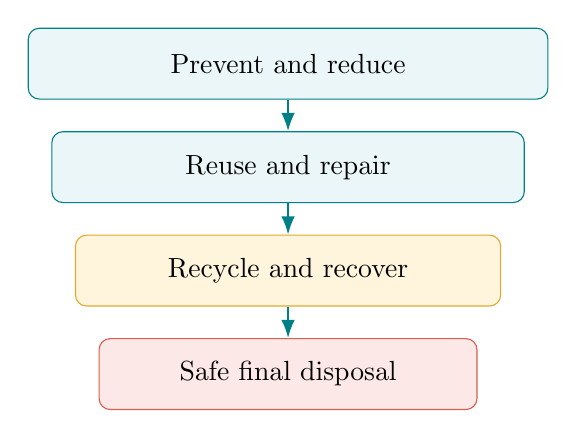
\begin{tikzpicture}[node distance=4mm,>=Latex]
\node[draw=Teal,fill=Pale,rounded corners,minimum width=66mm,minimum height=9mm,align=center] (p) {Prevent and reduce};
\node[draw=Teal,fill=Pale,rounded corners,minimum width=60mm,minimum height=9mm,align=center,below=of p] (r) {Reuse and repair};
\node[draw=Gold,fill=LightGold,rounded corners,minimum width=54mm,minimum height=9mm,align=center,below=of r] (c) {Recycle and recover};
\node[draw=Coral,fill=Rose,rounded corners,minimum width=48mm,minimum height=9mm,align=center,below=of c] (d) {Safe final disposal};
\draw[->,thick,Teal] (p)--(r);\draw[->,thick,Teal] (r)--(c);\draw[->,thick,Teal] (c)--(d);
\end{tikzpicture}
\end{center}
\textit{Figure 9.2.} A simple waste hierarchy: prevention comes before recycling and disposal.

\section{Electronic waste}
Computers, cables, printers, batteries and other electronic items should not be placed in ordinary waste when local rules require special handling. Use authorised collection or recycling channels, follow data-wiping and asset-disposal policies, and ensure that storage devices containing sensitive information are handled securely.

\section{Conserving energy and water}
Switch off equipment when it is not needed and when policy permits; use power-saving settings; maintain equipment; avoid unnecessary printing; repair leaks; and use water responsibly. Purchasing decisions can consider durability, repairability, energy use and end-of-life disposal, not only the initial price.

\section{Planning a small waste programme}
Start by observing what the workplace throws away and where the waste is produced. Set a realistic target, provide clearly labelled collection points, explain the process, identify an approved collection route and review results periodically. Do not mix separated waste after collection, and never handle unknown or hazardous material without the required training.

\par\noindent\textbf{Review Questions}\begin{enumerate}[label=\arabic*.,leftmargin=1.8em,itemsep=2pt,topsep=2pt]
\item Put the main waste-management options in preferred order.
\item Why does electronic waste need special attention?
\item List five ways to conserve resources in an office.
\item Outline a simple workplace recycling programme.
\end{enumerate}

\chapter{Diversity, Equality and Inclusive Workplaces}
An inclusive workplace makes it possible for people with different backgrounds, experiences and abilities to participate and contribute. Respect is shown through fair procedures, accessible communication, equitable opportunities and prompt action when discrimination or harassment occurs.

\section{Diversity and equality}
Diversity describes differences among people, including experience, culture, language, age, gender, disability and perspective. Equality means people are treated fairly and have equal rights and opportunities. Equity recognises that removing barriers may require different forms of support so people can participate meaningfully.

\section{Everyday inclusive behaviour}
Use respectful language, listen without interruption, avoid assumptions about a person's abilities or background, and give credit fairly. Meetings should make room for different voices. Work assignments, training, performance assessment and promotion should follow transparent and relevant criteria.

\section{Discrimination and harassment}
Discrimination involves unfair treatment linked to a protected or personal characteristic, according to applicable law and policy. Harassment can include unwelcome conduct that intimidates, humiliates or creates a hostile environment. Follow organisational reporting channels and relevant law. Bystanders should not escalate a situation; they can support the affected person and report concerns safely.

\section{Gender equality and work-life responsibilities}
Fair workplaces apply consistent standards, provide equal access to learning and advancement, and address barriers that prevent people from participating. Family responsibilities, caregiving and safety concerns should be handled through applicable policies and law rather than stereotypes about who should perform particular roles.

\section{Building an inclusive team}
Use clear selection criteria, accessible training material, fair performance feedback and a reliable process for raising concerns. Review workplace practices regularly. Inclusion is not achieved by a slogan; it requires people to notice barriers and improve the way work is organised.

\par\noindent\textbf{Review Questions}\begin{enumerate}[label=\arabic*.,leftmargin=1.8em,itemsep=2pt,topsep=2pt]
\item Explain the difference between equality and equity.
\item Give four examples of inclusive behaviour.
\item Why should hiring criteria be transparent?
\item What should a worker do if they experience or witness harassment?
\end{enumerate}

\chapter{Accessibility and Policies for Persons with Disabilities}
Accessibility means that people can use facilities, information, services and digital tools as independently as possible. A barrier may be physical, communicative, procedural or digital. Inclusive practice identifies barriers and makes reasonable adjustments in line with applicable law and workplace policy.

\photo{wheelchair-access.jpg}{Accessible workplace}{Figure 11.1. An accessible workplace considers clear space and practical access around desks. Photograph: David290, Wikimedia Commons, CC BY-SA 4.0.}
\section{Recognising different access needs}
People may have mobility, vision, hearing, learning, communication or other access requirements. Do not assume that everyone with the same disability needs the same support. Ask respectfully what adjustment is useful, protect privacy and involve the person in decisions that affect their work.

\section{Digital accessibility}
For websites and learning resources, use meaningful headings, descriptive link text, form labels, sufficient colour contrast, keyboard-accessible controls and alternative text for informative images. Do not communicate important information through colour alone. Captions and transcripts can help people who cannot hear audio; text alternatives can help people who cannot access a visual diagram.

\section{Physical and workplace adjustments}
Possible adjustments include accessible routes, suitable desk arrangements, assistive technology, flexible communication formats, adjusted work processes and accessible emergency information. The correct adjustment depends on the person, role, environment and applicable requirements. Keep routes clear and ensure emergency plans include people who may need assistance.

\section{Respectful support and privacy}
Speak directly to the person rather than only to a companion. Ask before offering physical assistance or moving mobility equipment. Do not disclose a person's disability or medical information without an appropriate basis. Apply workplace policies and relevant Indian law, including the Rights of Persons with Disabilities Act, 2016, where applicable; consult official guidance for current obligations.

\par\noindent\textbf{Review Questions}\begin{enumerate}[label=\arabic*.,leftmargin=1.8em,itemsep=2pt,topsep=2pt]
\item What is an accessibility barrier?
\item Give five examples of digital accessibility practices.
\item Why should adjustments be discussed with the person concerned?
\item How can a workplace improve emergency access for people with disabilities?
\end{enumerate}

\chapter{Integrated Case Study and Revision}
\section{Case study: a training-centre portal}
A training centre wants a portal to maintain learner details, course enrolments and marks. Staff need to add new learners, update records and generate course summaries. The portal will use PHP to process requests and MySQL to store data. The workplace also needs a safe workstation, inclusive user experience and a responsible plan for retiring old computers.

\section{Plan the database}
Identify entities such as learners, courses and enrolments. Assign primary keys and use foreign keys to represent relationships. Avoid storing repeated course details in every learner row. Decide which fields are required, which values need constraints and which reports are necessary.

\section{Plan the application}
Separate presentation, application logic and database access. Validate input on the server, use prepared statements, encode output and verify permissions for every sensitive action. Do not rely on hidden buttons or client-side checks to protect data. Keep credentials outside public source files and use a dedicated database account.

\section{Plan quality and workplace responsibility}
Write test cases for successful and invalid submissions, access control, database errors and responsive display. Review accessibility with keyboard navigation and readable labels. Organise the work area safely, report hazards, use energy-saving settings and send retired electronic equipment through an approved process.

\section{Revision questions}
\begin{enumerate}
\item Explain the role of a DBMS in a web application.
\item Compare primary keys and foreign keys.
\item Write SQL to retrieve students with marks above 70, ordered from highest to lowest.
\item Explain DDL, DML, DCL and transaction-control commands.
\item What is the purpose of SQL aggregate functions?
\item Describe how a PHP request can retrieve data from MySQL.
\item Explain how prepared statements help prevent SQL injection.
\item Compare indexed and associative PHP arrays.
\item What makes a function reusable and easy to test?
\item Define hazard and risk, and explain the hierarchy of controls.
\item Describe a responsible way to manage electronic waste.
\item Give examples of equality, equity and digital accessibility.
\end{enumerate}

\section{Answer-planning guide}
For definition questions, begin with a precise meaning and add one example. For comparison questions, explain the main difference and then compare practical uses. For code questions, state the purpose, show the syntax and describe any important safety condition. For workplace questions, identify the risk or barrier, propose a practical action and mention the relevant procedure or policy. These steps help produce clear, complete answers.

\end{document}
